\documentclass{article}
\usepackage{fancyhdr}
\usepackage{amsmath}
\usepackage{amssymb}
\usepackage{graphicx}
\usepackage{float}
\usepackage{subcaption}
\usepackage{hyperref}
\usepackage{listings}
\usepackage{color}
\usepackage{tikz}
\usepackage{pgfplots}
\usepackage{pgfplotstable}
\usepackage{listings}
\usepackage{color}

\definecolor{dkgreen}{rgb}{0,0.6,0}
\definecolor{gray}{rgb}{0.5,0.5,0.5}
\definecolor{mauve}{rgb}{0.58,0,0.82}

% Set up fancy header
\pagestyle{fancy}
\fancyhf{} % Clear default header and footer
\rhead{Keith Wesa} % Right header
\lhead{STAT 381 - Written Homework 1} % Left header
\rfoot{Page \thepage} % Right footer

\author{Keith Wesa}
\title{STAT 381 - Written Homework 1}
\date{\today}

\begin{document}

\section*{Problem 1}

\begin{itemize}
    \item[] \textbf{Problem 1:}  Alfred defines the sample space S to consist of all real numbers $x$ such that $2 < x \leq 8$. 
    We take two events in the sample space $B_1$ and $B_2$, where $B_1 = \{x |  2 < x \leq 4\}$ 
    and $B_2 = \{x | 3 < x \leq 5\}$.
\end{itemize}

\begin{figure}[H]
    \centering
    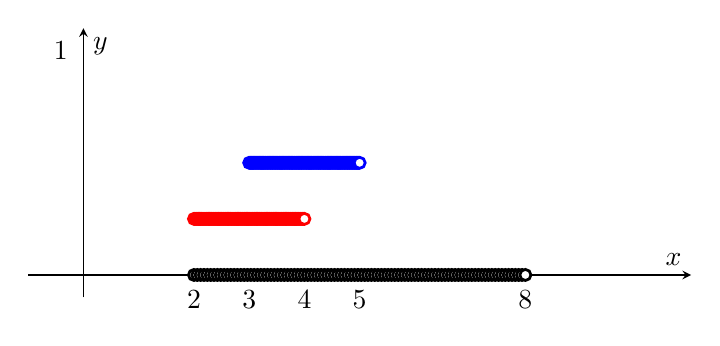
\begin{tikzpicture}
        \begin{axis}[
            xlabel={$x$},
            ylabel={$y$},
            xmin=0, xmax=10,
            ymin=0, ymax=1,
            axis lines=middle,
            xtick={2, 3, 4, 5, 8},
            ytick={-1, 1},
            xticklabels={$2$, $3$, $4$, $5$, $8$},
            yticklabels={$-1$, $1$},
            tick style={draw=none},
            enlargelimits=true,
            clip=false,
            width=10cm,
            height=5cm
        ]
        \addplot[domain=2:8, samples=100, color=black, line width=1pt, mark=*, mark options ={fill=white}] {0};
        \addplot[domain=2:4, samples=100, color=red, line width=1pt, mark=*, mark options={fill=white}] {.25};
        \addplot[domain=3:5, samples=100, color=blue, line width=1pt, mark=*, mark options={fill=white}] {.5};
        \end{axis}
    \end{tikzpicture}
\end{figure}

\begin{itemize}  
    \item[] \textbf{a)} Find the union of the two events $B_1$ and $B_2$.
    \begin{itemize}
        \item[] \textbf{Answer:} $B_1 \cup B_2 = \{x | 2 < x \leq 5\}$
    \end{itemize}
    \item[] \textbf{b)} Find the intersection of the two events inside the sample space.
    \begin{itemize}
        \item[] \textbf{Answer:} $B_1 \cap B_2 = \{x | 3 < x \leq 4\}$
    \end{itemize}
    \item[] \textbf{c)} Explain the errors in Alfred's calculations when they found the complement of $B_2$
    inside the sample space. Don't just state where the errors are, explain what the 
    correct statement should be. Hint: There are 3 errors.
    \begin{itemize}
        \item[] \textbf{Answer:} 
        \begin{itemize}
            \item[] \textbf{Error 1:} The first error is the set of numbers were given as $\mathbb{R}$ (real numbers).
            What Alfred did was give an answer as whole numbers, So he forgot to include the decimal numbers.
            \item[] \textbf{Error 2:} The second error is the answer should have been  something like this:
            \[
            B'_2 = \{x| 2 < x < 3 \cup 5 \leq x \leq 8\}
            \]
            
            \item[] This includes all real numbers.
            \item[]            
            \item[] \textbf{Error 3:} The third error is when they wrote out the equation they included the $3$.
        \end{itemize}
    \end{itemize}
\end{itemize}
\newpage
\section*{Problem 2}
    \begin{itemize}
        \item[] \textbf{Problem 2:} The Rotary Club in Kalamazoo holds an annual rubber duck race. Ducks are divided
        into four categories, $C_1$, $C_2$, $C_3$, and $C_4$. Each duck is a member of only one of these group, and 
        each duck is placed into a group. Overall, there are 1000 ducks that are in the race. There are 200 ducks in the 
        first category, 60 in the second category, 500 in the fourth category, and the remaining ducks are in the third category.
        \item[]
        \item[] Elizabeth sponsors 450 out of the 1000 ducks for the race. We are interested in the probablility that Elizabeth 
        sponsors 90 from the first category, 25 from the second category, 225 from the fourth category, and the remainder of the 
        450 ducks form the third category.
        \item[] \textbf{Questions to Answer:}
        \begin{itemize}
            \item[(a)] Show the Set up of the problem/calculations required to find the probablility required. No final answer is required.
            \item[] \textbf{Answer:}
            \begin{align*}
                P(C_1) &= \frac{90}{200} = \frac{2}{20}\\
                P(C_2) &= \frac{25}{60} = \frac{5}{12}\\
                P(C_3) &= \frac{[450 - (90 + 25 + 225)]}{[1000 - (200 + 60 + 500)]} = \frac{110}{240} = \frac{11}{24}\\
                P(C_4) &= \frac{225}{500} = \frac{9}{20}
            \end{align*}
        \item[(b)] Write R code to perform the calculation required in the previous part. Provide your code and your final answer from R.
        \item[] \newpage
        \item[] \textbf{Answer:}
        
        \begin{figure}[H]
            \centering
            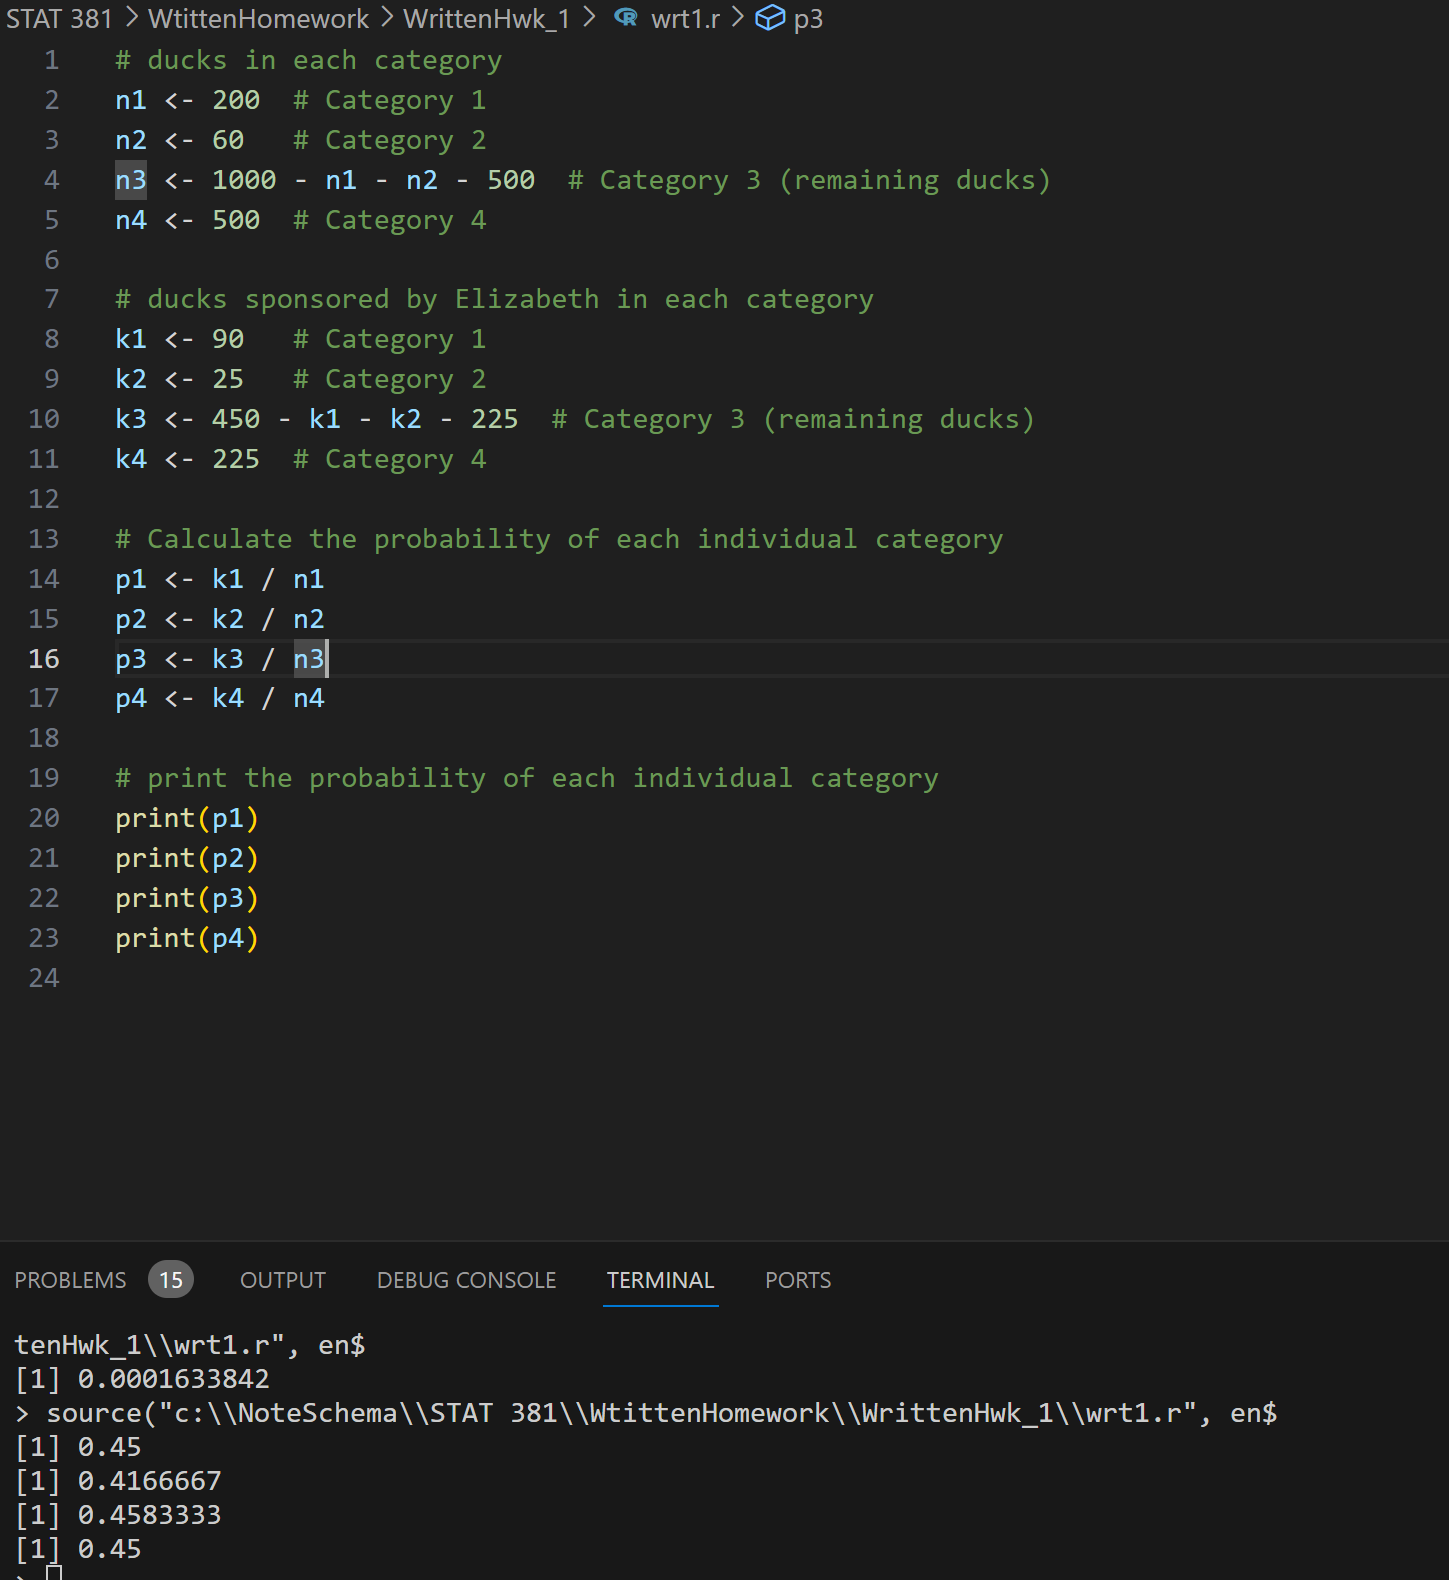
\includegraphics[width=10cm]{RCodehwk1.png}
        \end{figure}
        \item[] \newpage         
    
    \end{itemize}
    \end{itemize}
    \section*{Problem 3}   
    
    \begin{itemize}
        \item[] \textbf{Problem 3:} Suppose Francis can take one of two classes (statistics and econ). Francis knows the probablility that
        they pass each class. Francis is trying to calculate a conditional probablility, and is not sure which statement is true. Decide which 
        statement is true and explain why.
        \item[] \textbf{Option 1:} $1-P(\text{Fail}| \text{Econ}) = P(\text{Pass} | \text{Econ})$
        \item[] \textbf{Option 2:} $1-P(\text{Fail}| \text{Econ}) = P(\text{Fail} | \text{Econ})$
        \item[] \textbf{Option 3:} $1-P(\text{Fail}| \text{Econ}) = P(\text{Pass} | \text{Stat})$
        \item[] \textbf{Option 3:} $1-P(\text{Fail}| \text{Econ}) = P(\text{Fail} | \text{Stat})$
        \item[]
        \item[] \textbf{Answer:} Option 1 is true!
        \item[] \textbf{Explanation:} Relevant equations:
        \[
            1 - P(B|A) = P(B'|A)
        \]

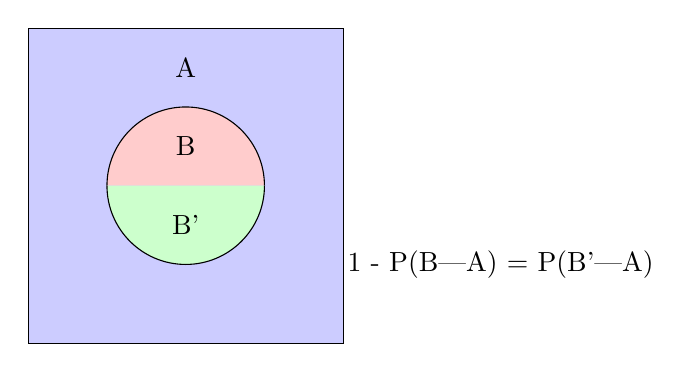
\begin{tikzpicture}
    % Square A
    \draw[fill=blue!20] (-2,0) rectangle (2,4);
    \node at (0,3.5) {A};
    
    % Semicircle B
    \draw[fill=red!20] (-1,2) arc (180:0:1);
    \node at (0,2.5) {B};
    
    % Semicircle B'
    \draw[fill=green!20] (1,2) arc (0:-180:1);
    \node at (0,1.5) {B'};
    
    % Equation
    \node at (4,1) {1 - P(B|A) = P(B'|A)};
\end{tikzpicture}
\newpage

\section{Problem 4:}
    
\begin{itemize}
    \item[] \textbf{Problem 4:} Melanie takes two events, $A$ and $B$. Assume that $P(A) \neq 0$ and $P(B) \neq 0$. Melanie wants
    to know if it is possible for these events to be both mutually exclusive and independent at the same time. Provide a mathematical
    example illustrating your viewpoint Your example should include:
    \begin{itemize}
        \item Definitions of the events $A$ and $B$. Either start with them mutually exclusive or as independent of each other.
        When you are constructing these events, make sure they meet the criteria for one mutually exclusive or independent.
        \item The probablility for $A$, and the probablility fo $B$.
        \item If you started with $A$ and $B$ as mutually exclusive, provide a a calculation to show if they are independent or not.
        \item If you started with $A$ and $B$ as independent, provide a calculation to show if they are mutually exclusive or not.
    \end{itemize}
    \item[] \textbf{Answer:}
    \item[] Start with $A$ and $B$ as mutually exclusive.
    \item[] \text{Definitions:}
    \item[] \textbf{Mutually Exclusive:} No shared outcomes.
    \[
        P(A \cap B) = \emptyset 
    \]
    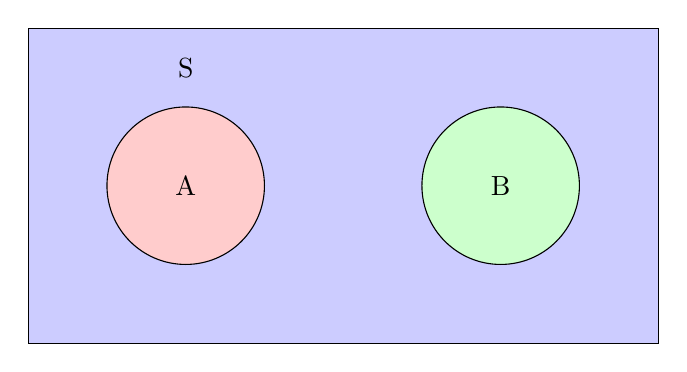
\begin{tikzpicture}
        \draw[fill=blue!20] (-2,0) rectangle (6,4);
        \node at (0,3.5) {S};
        
        
        \draw[fill=red!20] (1,2) arc (360:0:1);
        \node at (0,2) {A};
        
        
        \draw[fill=green!20] (3,2) arc (360:0:-1);
        \node at (4,2) {B};    
    \end{tikzpicture}
    \newpage
    \item[] \textbf{Independent:} The outcome of one event does not affect the outcome of the other event.
    \[
        P(A \cap B) = P(A)P(B)
    \]
    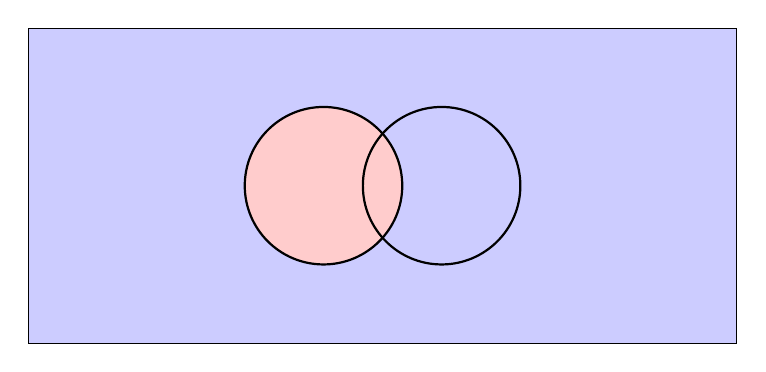
\begin{tikzpicture}
        \draw[fill=blue!20, opacity = 2] (-2,0) rectangle (7,4);
        \node at (0,3.5) {};
        
        
        \draw[thick,draw = black,fill=red!20, opacity = 2] (2.75,2) arc (360:0:1);
        \node at (0,2) {};
        
        
        \draw[thick, draw=black, opacity = 2] (2.25,2) arc (360:0:-1);
        \node at (4,2) {};    
    \end{tikzpicture}
    \item[] \textbf{Calculation:}
    \[
        P(A \cap B) = \emptyset \neq P(A)P(B)
    \]
    \begin{align*}
        P(A \cap B) &= P(A)P(B)\\
            \emptyset &= P(A)P(B)\\
            \emptyset &\neq P(A)P(B)
    \end{align*}
    \item[] \textbf{Conclusion:} Two events with $P(A) \neq 0$ and $P(B) \neq 0$ cannot be 
    both independent and mutually exclusive at the same time.
    \item[] $P(A \cap B) = \emptyset \neq P(A)P(B)$ So, $P(A \cap B) \neq \emptyset$  If $P(A) \neq 0$ and $P(B) \neq 0$ Which means that $A$ and $B$ would have value.
    Therefore $A$ and $B$ are not mutually exclusive.
    \item[] $P(A \cap B) = \emptyset \neq P(A)P(B)$ So, $P(A)P(B) > 0$ Which means that $A$ and $B$ are not mutually exclusive.
    \item[] If we were to assign we would have a non-zero probability of $P(A \cap B)$, which would mean that $A$ and $B$ are not mutually exclusive and independent.
    It would have to be either mutually exclusive or independent. By the way in which they are defined. 
    \begin{align*}
        \lnot\exists n \epsilon \mathbb{R} [(P(A) \lor P(B)) | P(A) \neq 0,  P(B) \neq 0] \\
    \end{align*}    
    


\end{itemize}





\end{itemize}

\end{document}